\section{Результаты анализа Монте-Карло моделирования эксперимента BM@N}

\subsection{Разрешение плоскости симметрии}

На рис.~\ref{fig:bmn_combinations} представлено разрешение плоскости симметрий $F1$, $F2$, $F3$ (слева направо)~\cite{Mamaev:2023yhz,Mamaev:2024}. 
Разрешение для плоскостей $F1$ и $F3$ было расчитано при помощи метода трёх подсобытий, которое выражается формулой (\ref{eq:r1_3sub}).
Для плоскости $F2$, которая не имеет достаточного разделения по псевдобыстроте с векторами $F1$ и $F3$, разрешение было рассчитано методом четырёх подсобытий (\ref{eq:r1_4sub}).
Аналогично, разрешение посчитанное с использованием комбинаций, не разделенных по быстроте $Q_1$-векторов (к примеру, $F1(F2,F3)$), отличается от значений рассчитанных при помощи комбинаций со значительным разделением по быстроте (к примеру, $F1(Tp,F3)$).
Значения $R_1$, полученные при помощи разделенных по быстроте комбинаций, согласуются между собой в пределах статистической ошибки для всех трех плоскостей симметрии. 
Значительное отличие разрешений, полученных с использованием комбинаций не разделенных по быстроте $Q_1$-векторов, может быть объяснено распространением адронного ливня в поперечном направлении, что вызывает дополнительные корреляции между векторами $F1$ и $F2$, и $F1$ и $F3$.
%
\begin{figure}[ht]
\begin{center}
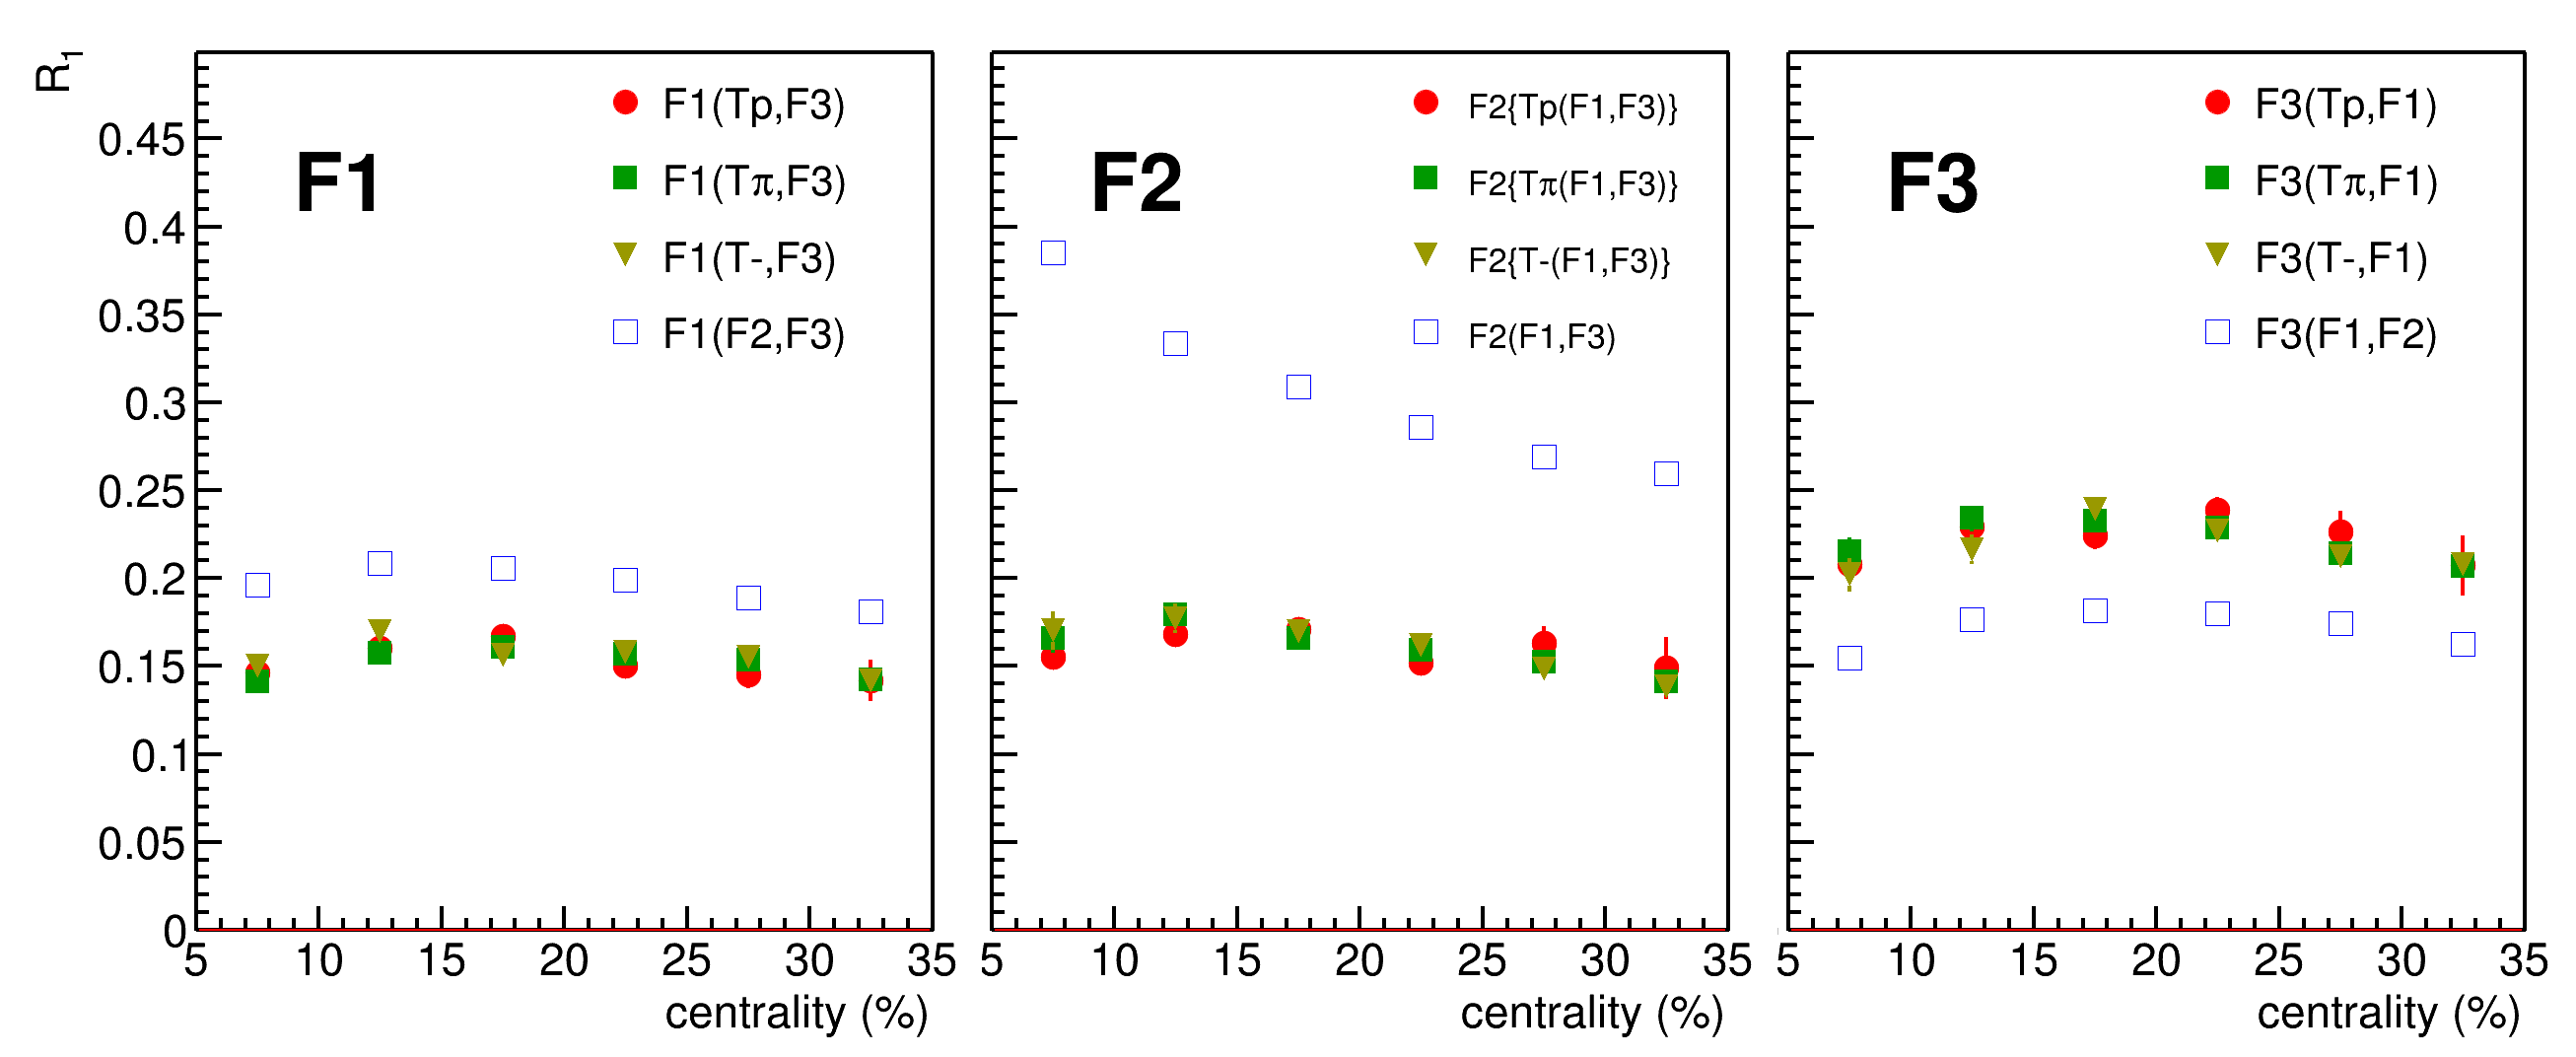
\includegraphics[width=0.95\linewidth]{images/R1_F123_combinations_centrality.png}
\caption{Разрешение плоскостей симметрии слева: $F1$, посередине: $F2$, справа: $F3$. Различные маркеры и цвета обозначают комбинации $Q_1$-векторов, использованных для расчета разрешения плоскости симметрии.}
\label{fig:bmn_combinations}
\end{center}
\end{figure}

\subsection{Производительность установки BM@N для измерения направленного и эллиптического потоков}

На рис.~\ref{fig:bmn_v1_v2} слева представлен направленный поток протонов, как функция быстроты в Монте-Карло моделировании столкновений Xe~+~Cs из модели JAM~\cite{Mamaev:2023yhz,Mamaev:2024}. 
На рис.~\ref{fig:bmn_v1_v2} справа показан эллиптический поток протонов, как функция поперечного импульса в Монте-Карло моделировании столкновений Xe~+~Cs из модели JAM. 
Разными цветами обозначена разная энергия столкновений. 
Линии обозначают $v_1$ и $v_2$ извлеченные напрямую из модели без реконструкции. 
Маркерами обозначены результаты анализа Монте-Карло моделирования отклика детектора.
Между данными извлеченными из модели и результатами анализа после реалистичной цепочки реконструкции наблюдается согласие в пределах статистической ошибки. 
%
\begin{figure}[ht]
\begin{center}
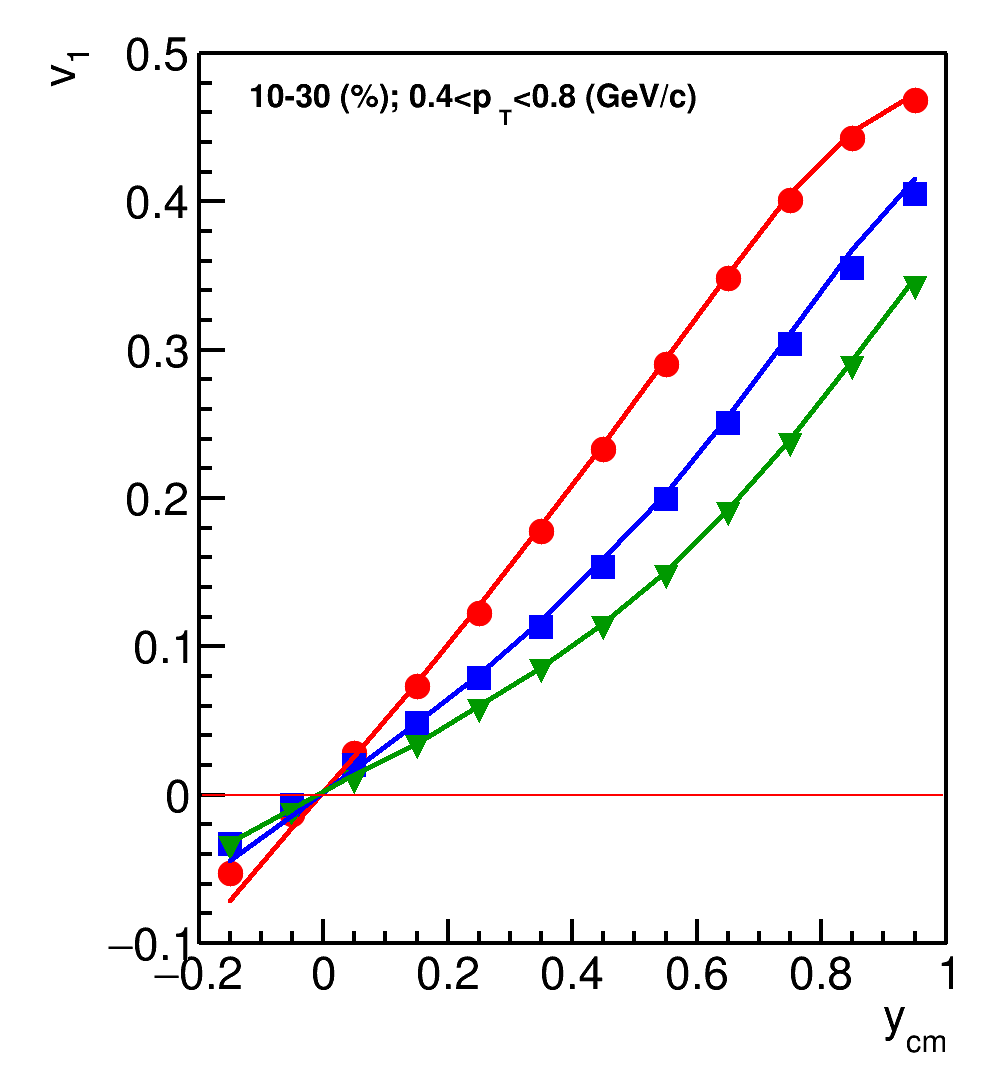
\includegraphics[width=0.45\linewidth]{images/v1_proton_tof_rapidity.png}
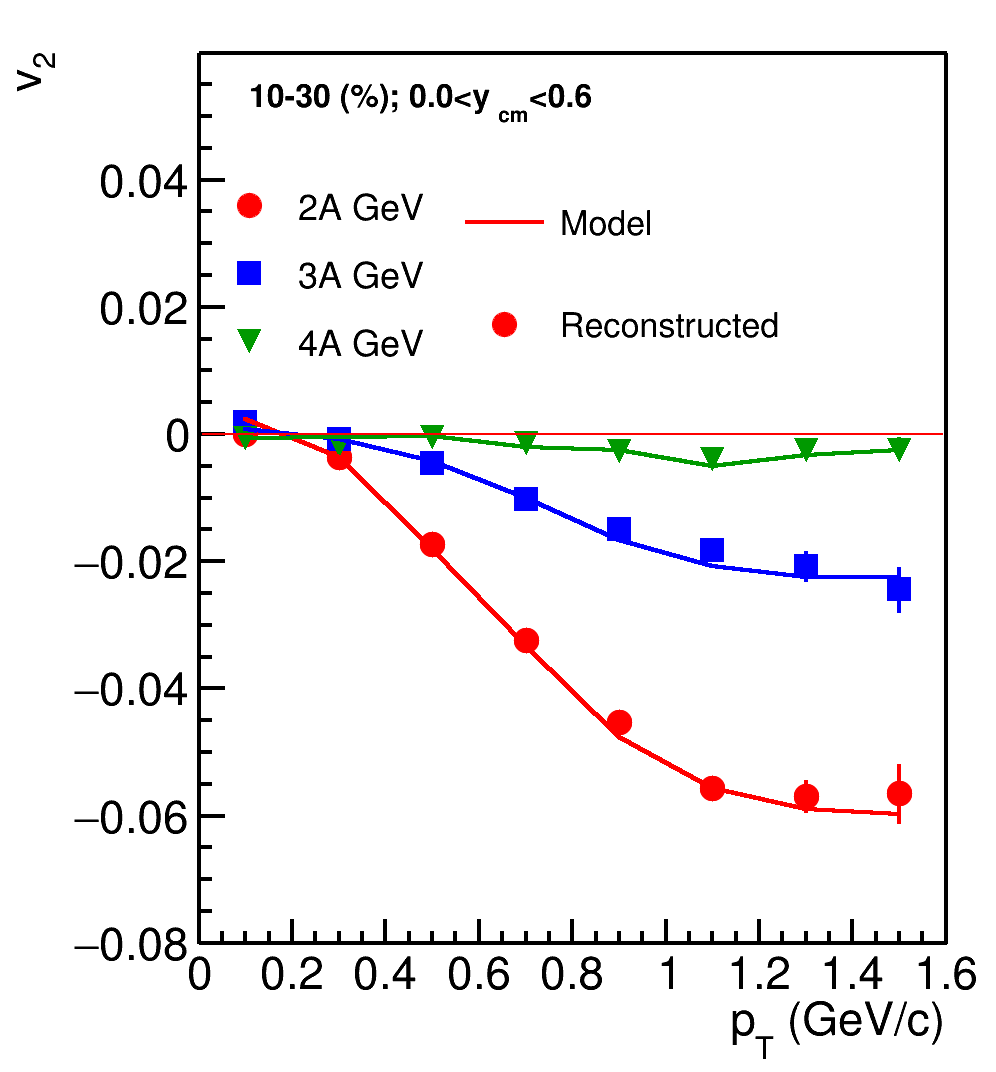
\includegraphics[width=0.45\linewidth]{images/v2_proton_tof_pT.png}
\caption{ 
    Направленный (слева) и эллиптический (справа) поток протонов как функция быстроты и поперечного импульса соответственно в Монте-Карло моделировании столкновений $Xe+Cs$ из модели JAM. Разными цветами обозначена разная энергия столкновений. Линии обозначают $v_1$ и $v_2$ извлеченные напрямую из модели без реконструкции. Маркерами обозначены результаты анализа Монте-Карло моделирования отклика детектора.
}
\label{fig:bmn_v1_v2}
\end{center}
\end{figure}

\subsection{Разрешение плоскости симметрии из данных}

В начале 2023 года на устновке BM@N закончиался набор данных столкновений ядер Xe~+~CsI при энергии $E_{kin}=3.8A$~ГэВ.
Методики, отработанные на Монте-Карло моделировании установки были использованы для восстановления плоскости симметрии в экспериментальных данных.
Модули детектора FHCal были разделены на 3 группы: F1, F2 и F3.
Для оценки систематики, связанной с непотоковыми корреляциями были введены 2 вектора из треков заряженных частиц:
\begin{itemize}
    \item T+: положительно заряженные частицы с поперечным импульсом $p_T > 0.2$~ГэВ/c и псеводобыстротой $2<\eta<3$;
    \item T-: отрицательно заряженные частицы с поперечным импульсом $p_T > 0.2$~ГэВ/c и псеводобыстротой $1.5<\eta<3$.
\end{itemize}

C помощью формулы (\ref{eq:r1_3sub}) методом трех подсобытий было получено разрешение для плоскостей симметрии $F1$, $F2$ и $F3$.
Разрешение было вычислено, используя различные комбинации $Q_1$-векторов.
Дополнительно, для подсобытия $F2$, были получены оценки методом четырёх подсобытий, который выражается формулой (\ref{eq:r1_4sub}).
Разрешение плоскости симметрии как функция центральности из экспериментальных данных представлено на рис.~\ref{fig:bmn_r1_data}.
Для всех плоскостей симметрии все три комбинации находятся в хорошем согласии, что говорит о малом вкладе непотоковых корреляций.

\begin{figure}[ht]
\begin{center}
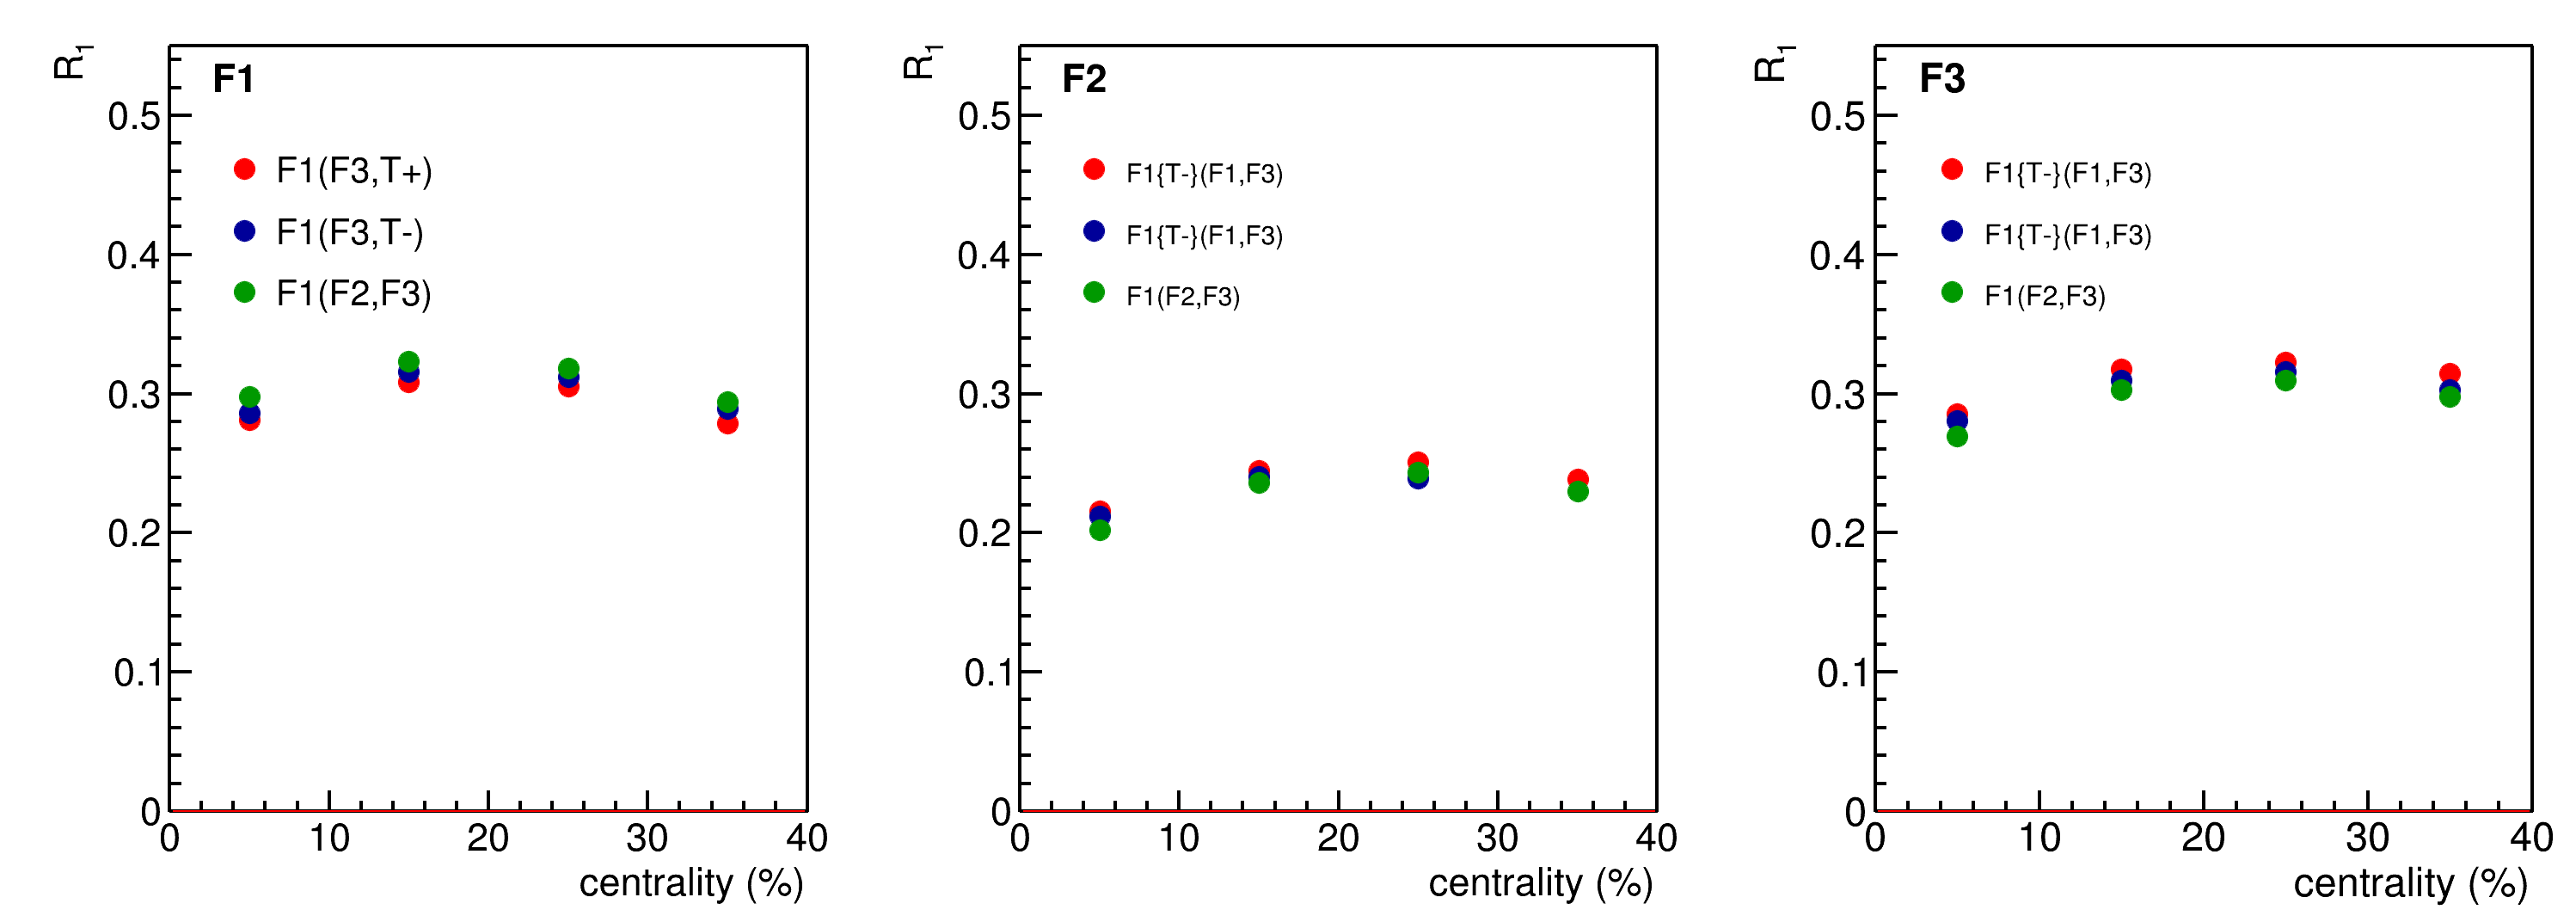
\includegraphics[width=0.95\linewidth]{images/F123_centrality.png}
\caption{ 
    Разрешение плоскостей симметрии F1, F2 и F3 справа налево как функция центральности из экспериментальных данных столкновений Xe~+~CsI при энергии $3.8A$~ГэВ на BM@N.
}
\label{fig:bmn_r1_data}
\end{center}
\end{figure}

\section{Выводы к главе 4}
В главе приводятся результаты измерения направленного потока в столкновениях Au+Au при энергии 1.23$A$~ГэВ и Ag+Ag при энергиях 1.23 и 1.58$A$~ГэВ в эксперименте HADES.
Результаты для $v_1$ протонов согласуются с опубликованными коллаборацией HADES.
В главе обсуждаются свойства масштабирования направленного потока протонов $v_1$ с энергией столкновений и размером системы.
Обнаружено, что направленный поток протонов не зависит от энергии столкновений и размера системы в столкновениях Au+Au при энергии 1.23$A$~ГэВ и Ag+Ag при энергиях 1.23 и 1.58$A$~ГэВ в эксперименте HADES.
Значения наклона направленного потока $dv_1/dy$ после коррекции на размер системы и быстроту пучка описываются универсальной зависимостью от относительного прицельного параметра.
Наклон направленного потока $dv_1/dy$ в столкновениях Au+Au при энергии 1.23$A$~ГэВ и Ag+Ag при энергиях 1.23 и 1.58$A$~ГэВ в эксперименте HADES хорошо согласуется с мировыми данными.
В главе представлены результаты исследования Монте-Карло моделирования эксперимента BM@N на возможность измерения направленного и эллиптического потока в первом физическом сеансе установки.
Используя методы, апробированные на экспериментальных данных набранных на установке HADES, была разработа физическая программа измерения коллективной анизотропии в эксперименте BM@N.